\documentclass{memoir}
\usepackage[T1]{fontenc}
\usepackage[utf8]{inputenc}
\usepackage{hyperref}
\usepackage[english,italian]{babel}
\usepackage{tikz}
\usetikzlibrary{automata,positioning,topaths,calc,arrows.meta,shapes.geometric}
\usepackage{amssymb}
\usepackage{amsmath}
\usepackage[italian]{cleveref}
\usepackage[italiano,ruled, linesnumbered]{algorithm2e}
\usepackage{minted}


\title{Implementazione di un sistema di incrocio stradale intelligente \\ for the Project of Distributed Systems}

\author{Tiziano Mele\\Valentino Picotti\\DMIF, University of Udine, Italy}

\date{Version 1, \today}

\begin{document}


%\begin{titlingpage}
\maketitle
\begin{abstract}
  Un sistema di incrocio stradale intelligente vuole essere una soluzione al
  problema della congestione stradale. Con l'avvento dei sistemi wireless e
  autonomici ci si chiede se sia possibile per i veicoli stradali poter decidere
  direttamente tra di loro chi debba impegnare l'incrocio. Di seguito si indaga
  una soluzione che permetta di eliminare le lanterne semaforiche in modo da
  ridurre i tempi medi di attesa dei veicoli in coda.
\end{abstract}
%\end{titlingpage}

\chapter{Introduzione}\label{ch:intro}

La soluzione che viene proposta in questo lavoro vuole essere di tipo
distribuito, dove i singoli veicoli sono entità indipendenti e con conoscenza
parziale dell'ambiente circostante data dalla sensoristica di bordo. Compito dei
veicoli è quello di formare una rete peer-to-peer che permetta loro di
comunicare autonomamente, senza bisogno di un server centrale.

% TODO: Da riconsiderare per capitolo 3.1
% Inoltre la soluzione mira ad essere fisicamente plausibile, ipotizzando un
% deploy in una situazione reale (o mondo reale)
% soluzione fisicamente plausibile
% al funzionamento fisico della sensoristica
% Molte scelte sono state effettuate pensando al livello tecnologico della
% sensoristica ad oggi disponibile; ad esempio è stato tenuto conto del fatto che
% i dispositivi wireless hanno un raggio di azione limitato.

I principali requisiti che si vogliono soddisfare sono:
\begin{description}
\item[Sicurezza stradale] Le auto che attraversano l'incrocio non devono
  scontrarsi.
\item[Liveness] Ogni macchina che si trova ad un incrocio deve prima o poi
  attraversarlo.
\item[Fairness] Quando un'auto chiede di impegnare l'incrocio, esiste un tempo
  limite entro cui le viene assegnato.
\item[Deadlock freedom] Non possono verificarsi situazioni in cui nessuna
  macchina nell'incrocio può muoversi.
\item [Fault Tolerance] Il sistema deve funzionare in caso di guasti fisici o
  logici. Un guasto fisico comporta che la macchina è attiva nella rete ma non
  può muoversi. Un guasto logico comporta che la macchina non è più
  raggiungibile nella rete, ma comunque presente fisicamente nell'ambiente.
\item [Distribuito] Le macchine si parlano tra di loro senza un server centrale
  che potrebbe diventare un SPOF.
\item [Generale] E' possibile utilizzare il sistema su un qualsiasi tipo di
  incrocio: è sufficiente cambiare il grafo di descrizione dell'incrocio (non è
  necessario agire modificando la struttura del sistema e degli algoritmi).
\end{description}

\subsection{Struttura complessiva dell'implementazione}

Lo spazio fisico è partizionato in una griglia dove ogni macchina può occupare
al più una cella. La griglia è poi rappresentata da un grafo orientato e pesato
in cui i nodi rappresentano le singole celle della griglia. Si ha una collisione
quando due auto vanno ad occupare la stessa cella nella griglia (lo stesso nodo
del grafo). Le macchine sono dotate di sensori di prossimità, gps e un modulo
wifi per comunicare con le altre macchine. Una macchina può avanzare solo se il
sensore di prossimità non rileva ostacoli ed è in grado di capire se si trova in
prossimità di un incrocio mediante il modulo gps. In quest'ultimo caso prima di
avanzare deve coordinarsi con eventuali altre macchine presenti. Il
coordinamento si traduce in una fase di elezione di un leader dell'incrocio, che
poi deciderà quali macchine far passare.


Per testare il sistema è stato implementato un ambiente simulato le cui
funzionalità rispecchino il più possibile quelle di un ambiente reale.

\chapter{Analisi}\label{ch:analysis}
In questo capitolo si descrivono requisiti funzionali e non funzionali della
soluzione fornita.

\section{Requisiti funzionali}

Al fine di poter fornire una simulazione realistica, sono stati individuati i
seguenti requisiti funzionali per gli attori che vi partecipano.

\subsection{Veicolo}

Un veicolo deve soddisfate i seguenti requisiti funzionali:
\begin{itemize}
\item Muoversi in autonomia
\item Poter interrogare i sensori di prossimità
\item Conoscere la sua posizione gps attuale e più in generale conoscere il suo
  intero tragitto
\item Riconoscere quando si trova in prossimità di un incrocio, al suo interno o
  se sta percorrendo un tratto senza incroci
\item Riconoscere eventuali macchine guaste che ostacolino il suo percorso
\item Richiedere l'intervento del carro attrezzi per i veicoli che suppone
  essere guasti
\item Disporre di un meccanismo di comunicazione broadcast per poter comunicare
  con le auto nelle vicinanze
\item Disporre di un meccanismo di comunicazione unicast che permetta di
  comunicare con una singola auto
\item Essere in grado di coordinarsi con gli altri veicoli per attraversare
  l'incrocio
\end{itemize}

\subsection{Ambiente}

L'ambiente è l'unico attore che dispone della conoscenza globale dell'incrocio,
compresa la posizione esatta di ogni auto. Deve quindi soddisfare i seguenti
requisiti:
\begin{itemize}
\item Conoscere la posizione esatta di ogni veicoli
\item Rispondere alle richieste dei sensori di prossimità dei veicoli
\item Simulare la comunicazione broadcast inoltrando il messaggio ai soli
  veicoli a portata wireless del mittente
\item Simulare l'intervento del carro attrezzi a seguito di una richiesta di
  intervento da parte di un veicolo
\end{itemize}

La struttura dell'incrocio oltre che fornire una descrizione topologica e
spaziale deve anche indicare le traiettorie di percorrenza ammesse. Tale
struttura la si considera come dato di input della simulazione.

\subsection{Interfaccia grafica}

La soluzione prevede la presenza di un interfaccia grafica dalla quale è
possibile visualizzare ad ogni istante lo stato dell'incrocio per monitorarne il
funzionamento e aggiungere nuovi veicoli alla simulazione.


\section{Requisiti non funzionali}
I requisiti non funzionali che una soluzione deve soddisfare sono:
\begin{description}
\item[Sicurezza stradale] Le auto che attraversano l'incrocio non devono
  scontrarsi.
\item[Liveness] Ogni macchina che si trova ad un incrocio deve prima o poi
  attraversarlo.
\item[Fairness] Quando un'auto chiede di impegnare l'incrocio, esiste un tempo
  limite entro cui le viene assegnato.
\item[Deadlock freedom] Non possono verificarsi situazioni in cui nessuna
  macchina nell'incrocio può muoversi.
\item[Near real-time] È necessario imporre un limite di tempo all'esecuzione
  della fase di coordinamento, che deve avvenire in \emph{near real-time} per
  scongiurare fermate prolungate ai veicoli.
\end{description}

Inoltre la soluzione soddisfa le seguenti trasparenza:
\begin{description}
\item[Access transparency] Non c'è un concetto di risorsa remota a cui le
  macchine accedono. Le macchine utilizzano dati ricavati da sensori oppure
  messaggi ricevuti da altre macchine.
\item[Location transparency] Una macchina comunica con i vicini senza conoscerne
  la loro posizione fisica nell'ambiente.
\item[Concurrency transparency] Più macchine possono impegnare l'incrocio senza
  interferire l'una con l'altra.
\item[Failure transparency] Sono ammessi fallimenti fisici e logici delle
  macchine in un qualsiasi momento. Se la macchina si guasta fisicamente è lei
  stessa a ``chiamare il carro attrezzi''; se la macchina si guasta logicamente,
  è la macchina dietro che, passato un certo intervallo di tempo, chiede
  l'intervento di un carro attrezzi. Dovesse guastarsi il leader dell'incrocio,
  si procede con l'elezione di un nuovo leader.
\item[Mobility transparency] Il coordinamento funziona a prescindere dalla
  posizione del leader, che può essere uno qualsiasi fra i veicoli presenti.
\end{description}


%Come primo passaggio viene creato un processo "environment" dove viene salvato
%lo stato globale dell'incrocio. L'incrocio viene tradotto in un grafo orientato
%pesato, dove ogni nodo conterrà le seguenti informazioni:
%\begin{itemize}
%\item Nome
%\item Tipologia di nodo: TailNode(Nodo in coda) TopNode (Nodo in prossimità di
%  un incrocio) CrossNode(Nodo incrocio)
%\item Elenco di macchine che occupano il nodo stesso
%\end{itemize}
%Il peso degli archi del grafo viene assegnato in base alla distanza fisica tra i
%due nodi.
%Questo modulo viene interrogato dalle varie macchine per simulare dati relativi
%alla sensoristica.
%
%Ogni veicolo sarà implementato come un processo che quindi potrà interrogare i
%sensori per ottenere le informazioni su posizione, ostacoli, percorso più breve
%verso la sua destinazione.
%
%Le macchine sono in relazione client-server con l'environment. Ogni automobile è
%una macchina a stati finiti per la quale si prevede di utilizzare il behaviour
%di erlang gen\_statem. Gli stati principali per un veicolo sono:
%\begin{itemize}
%\item \texttt{INQUEQUE}: La macchina si trova in questo stato quando è in coda
%  (non è la prima macchina della fila)
%\item \texttt{DISCOVER}: La macchina è la prima della file. In questo stato la
%  macchina manda un broadcast per scoprire le auto vicine.
%\item \texttt{ELECTION}: La macchina è la prima della fila. E' in corso
%  l'elezione di un leader dell'incrocio
%\item \texttt{SLAVE}: L'elezione si è conclusa e la macchina non è leader. Mando
%  il mio percorso al leader e attendo risposta "verde"/"rosso".
%\item \texttt{M-FETCH}: La macchina è stata eletta leader dell'incrocio. Attendo
%  i percorsi delle macchine SLAVE.
%\item \texttt{M-COORD}: In base ai percorsi e alle priorità delle macchine mando
%  messaggi "verde"/"rosso" agli SLAVE.
%\item \texttt{CROSSING}: La macchina è in questo stato se si trova su un nodo
%  del grafo di tipo CrossNode.
%\item \texttt{PH-FAULT}: La macchina ha un guasto fisico.
%\end{itemize}
%
%Ogni veicolo può ricevere uno dei seguenti eventi:
%\begin{itemize}
%\item \texttt{disc}: La macchina è appena arrivata in prossimità dell'incrocio e
%  manda in broadcast un "discover" con il suo pid e il suo percorso. A livello
%  pratico per simulare il broadcast il messaggio di discover viene mandato
%  all'environment che poi rigira alle altre macchine. Queste quindi a loro volta
%  mandano un messaggio di "hellofrom" alla nuova macchina (con il loro
%  percorso).
%\item \texttt{disc\_tm}: lo stato \texttt{DISCOVER} ha un suo timeout. Una volta
%  trascorso viene innescato questo evento.
%\item \texttt{wait(tag:*)}: se la macchina si trova in stato \texttt{DISCOVER} e
%  riceve questo evento rimane nello stato \texttt{DISCOVER} e resetta il
%  timeout.
%\item \texttt{hello(pid)}: se la macchina si trova in stato \texttt{DISCOVER},
%  mi salvo il pid ricevuto tra i conosciuti.
%\item \texttt{elect}: Messaggio di \emph{election} dell'algoritmo bully.
%\item \texttt{coord}: Messaggio di \emph{coordinator} dell'algoritmo bully.
%\item \texttt{ans}: Messaggio di \emph{answer} dell'algoritmo bully.
%\item \texttt{elect\_tm}: Evento di timeout (elezione fallita) dell'algoritmo bully.
%\item \texttt{route}: messaggio contenente id, priorità, lista macchine con cui
%  è in conflitto.
%\item \texttt{route\_tm}: evento di timeout per lo stato \texttt{M-FETCH}.
%\item \texttt{green}: Messaggio che notifica a macchina in stato \texttt{SLAVE}
%  che può attraversare incrocio.
%\item \texttt{red}: Messaggio che notifica a macchina in stato \texttt{SLAVE}
%  che non può attraversare incrocio.
%\item \texttt{gr\_timeout}: evento di timeout per lo stato \texttt{SLAVE} e
%  \texttt{M-COORD}.
%\end{itemize}
%
%\begin{figure}
%  \centering
%  \begin{tikzpicture}[shorten >=1pt, node distance=2.5cm,on grid,auto, bend
%    angle=30, font=\footnotesize\ttfamily]
%    \node[state,initial] (queue) {INQUEUE};%
%    \node[state] (disc) [right=of queue] {DISCOVER};%
%    \node[state] (elec) [right=of disc,xshift=0.5cm] {ELECTION};%
%    \node[state] (slave) [xshift=1cm,above right=of elec] {SLAVE};%
%    \node[state] (m-fetch) [xshift=1cm,below right=of elec] {M-FETCH};%
%    \node[state] (m-coord) [right=of m-fetch,xshift=0.5cm] {M-COORD};%
%    \node[state] (cross) [above right=of m-coord] {CROSSING};%
%    \node[state,initial,initial text=fault] (fault) [below=of disc]
%    {PH-FAULT};%
%    \path[->]%
%    (queue) edge node {on\_top} (disc)%
%    (disc) edge [loop above] node[xshift=-0.2cm] {disc,hello,wait} ()%
%    edge node {disc\_tm} (elec)%
%    edge [bend right] node[yshift=-0.5cm] {elec} (elec)%
%    edge [bend left] node[yshift=0.1cm,xshift=0.7cm] {coord} (slave)%
%    (elec) edge [loop below] node {disc,elect,ans} ()%
%    edge node {coord} (slave)%
%    edge [bend right] node[yshift=0.45cm] {elec\_tm} (disc)%
%    edge node[xshift=-0.4cm,yshift=0.2cm] {master} (m-fetch)%
%    (slave) edge [loop
%    above] node {disc} () edge node {green} (cross) edge [bend right=50]
%          node[xshift=-0.5cm,yshift=0.7cm] {red,gr\_tm} (disc) (m-fetch) edge
%          [loop above] node {route,disc} () edge node {route\_tm} (m-coord)
%          (m-coord) edge [loop above] node {disc,route} () edge [below] node
%          [xshift=0.5cm] {green} (cross) edge [bend left=50] node {red,gr\_tm}
%          (disc) (cross) edge [loop above] node {disc} ();
% \end{tikzpicture}
% \caption{Car: Finite State Machine}
%\end{figure}
%
%Ogni veicolo ha un suo valore di priorità iniziale, che viene incrementato ogni
%volta che il veicolo riceve il messaggio \texttt{red} (lo può ricevere solo se è
%in stato \texttt{SLAVE} o \texttt{M-COORD}). Il leader dell'incrocio decide chi
%far passare nel seguente modo:
%\begin{itemize}
%\item Ordina le macchine per priorità;
%\item Farà sicuramente passare la prima.
%\item Calcola un insieme massimale di macchine indipendenti rispetto alla prima
%\end{itemize}

\chapter{Progetto}

\section{Architettura Logica}
\label{sec:arclog}
Le componenti principali della soluzione sono:
\begin{itemize}
\item Modulo Veicolo: utilizzato per rappresentare il singolo veicolo;
\item Modulo Environment: utilizzato per rappresentare l'ambiente e simulare
  l'interazione del veicolo con la sensoristica;
\item Interfaccia grafica: modulo utilizzato per monitorare e interagire con
  l'ambiente.
\end{itemize}

Di seguito vengono descritte nel dettaglio le funzionalità implementate da ogni componente
\subsection{Veicolo}
Ogni veicolo è una macchina a stati finiti il cui output dipende dallo stato
attuale e dagli eventi in input. È naturale, quindi, descrivere un veicolo come
una macchia di Mealy, in cui gli input sono generici eventi e gli output sono
messaggi inviati. Gli stati principali per un veicolo sono:
\begin{itemize}
\item \texttt{INQUEUE}: Il veicolo si trova in questo stato quando stà
  transitando in una zona non in prossimità di un incrocio;
\item \texttt{DISCOVER}: Il veicolo si trova in prossimità di un incrocio e deve
  effettuare il \emph{discover} delle auto nelle vicinanze;
\item \texttt{WAIT}: Il veicolo deve attendere il completamento di un'elezione
  già in corso o il transito di altri veicoli nell'incrocio;
\item \texttt{ELECTION}: Il veicolo si trova in prossimità di un incrocio e sta
  partecipando all'elezione di un leader;
\item \texttt{SLAVE}: L'elezione si è conclusa e il veicolo non è leader. Rimane
  quindi in attesa di istruzioni da parte del leader;
\item \texttt{MASTER}: Il veicolo è stato eletto leader dell'incrocio, quindi
  procede inviando istruzioni ai veicoli \texttt{SLAVE};
\item \texttt{CROSSING}: Il veicolo sta percorrendo l'incrocio;
\item \texttt{PH-FAULT}: Il veicolo ha rilevato un guasto fisico. Un guasto
  fisico può avvenire in un qualsiasi momento.
\end{itemize}

Per ogni stato si elencano gli eventi che il veicolo è tenuto a gestire, come ad
esempio messaggi ricevuti o timer interni, e le azioni intraprese allo scaturire
di tali eventi. Gli eventi non menzionati in un certo stato vanno ignorati.

\paragraph{\texttt{INQUEUE}}
Il veicolo avanza di una cella nello spazio fisico ogni \emph{n} secondi
seguendo la sua rotta e rallentando nel caso in cui il sensore di prossimità
rilevi un ostacolo oppure giunga in prossimità dell'incrocio.

\begin{figure}[h]
  \centering
  \begin{tikzpicture}[shorten >=1pt, node distance=2.5cm,on grid,auto, bend
    angle=30, font=\footnotesize\ttfamily]
    \node[state,initial, initial text=enter/\_] (queue) {INQUEUE};%
    \node[state] (disc) [right=of queue, xshift=1cm] {DISCOVER};%
    \path[->] (queue) edge [loop above] node[align=center]%
    {car\_mv/\_\\fault/no} ()%
                      edge node {car\_mv/\_} (disc);%
  \end{tikzpicture}
\end{figure}

L'evento \texttt{car\_mv} rappresenta l'avanzamento del veicolo lungo la sua
rotta. Alla ricezioni di questo evento il veicolo interroga il sensore di
prossimità: se vi sono ostacoli, il veicolo si ferma in attesa di un nuovo
evento \texttt{car\_mv}; se la strada è libera procede con la sua corsa fino ad
occupare la cella successiva nella griglia. A questo punto, se la nuova cella
risulta essere in prossimità di un incrocio, il veicolo entra nello stato
\texttt{DISCOVER}, altrimenti rimane nello stato \texttt{INQUEUE} in attesa di
un nuovo evento \texttt{car\_mv}.

Se il veicolo rileva un ostacolo che lo obbliga a una fermata prolungata, avvia
una chiamata al soccorso stradale in merito alla posizione dell'ostacolo. Sarà
poi il soccorso stradale a rimuovere l'eventuale veicolo dalla posizione
segnalata, se effettivamente guasto. Il soccorso stradale è una funzionalità
offerta dal modulo \emph{Environment}.

\paragraph{\texttt{DISCOVER}}
In prossimità di un incrocio il veicolo deve capire se vi siano altri veicoli in
prossimità dello stesso incrocio. Viene quindi applicato il protocollo di
\emph{discovery} descritto nella \cref{sec:protalg}.

\begin{figure}[h]
  \centering
  \begin{tikzpicture}[shorten >=1pt, node distance=2.5cm,on grid,auto, bend
    angle=30, font=\footnotesize\ttfamily]
    \node[state, initial, initial text=enter/disc] (disc) {DISCOVER};%
    \node[state] (elec) [above right=of disc,xshift=2.5cm] {ELECTION};%
    \node[state] (slave) [xshift=2.5cm,below right=of disc] {SLAVE};%
    \node[state] (wait) [below=of disc] {WAIT};%
    \path[->] (disc) edge [loop above] node[align=center]
    {disc/hello\\hello/\_\\fault/no} ()%
    edge node[align=center, xshift=0.7cm,yshift=0.2cm] {disc\_tm/\_\\elect/\_} (elec)%
    edge node {wait/\_} (wait)%
    edge node {coord/\_} (slave);%
  \end{tikzpicture}
\end{figure}
Quando il veicolo entra nello stato \texttt{DISCOVER} invia il messaggio
broadcast \texttt{disc}, che verrà ricevuto dai soli veicoli a portata wireless,
contenente la propria identità e la propria rotta. Rimane poi in attesa dei
seguenti messaggi fino allo scadere di un timeout (evento \texttt{disc\_tm}):
\begin{itemize}
\item \texttt{disc}: Un altro veicolo ha segnalato la sua presenza
  nell'incrocio. Il veicolo memorizza le informazioni sul mittente e risponde
  con un messaggio \texttt{hello} per segnalare la propria presenza.
\item \texttt{hello}: Ricevuto in risposta a un \texttt{disc}; il veicolo
  memorizza le informazioni sul mittente.
\item \texttt{wait}: Ricevuto in risposta a un \texttt{disc} quando un elezione
  è già in corso o un veicolo sta impegnando l'incrocio. Il veicolo entra nello
  stato \texttt{WAIT} per un breve periodo prima di ritornare nella fase di
  \emph{discovery}.
\item \texttt{elect}: Un altro veicolo ha indetto un'elezione. Il veicolo entra
  nello stato \texttt{ELECTION} per partecipare all'elezione.
\item \texttt{coord}: Un altro veicolo è stato eletto il leader dell'incrocio.
  Il veicolo memorizza l'identità del leader e entra nello stato \texttt{SLAVE}.
\item \texttt{fault}: Il soccorso stradale ha richiesto lo stato del veicolo.
  Non essendoci anomalie, viene inviata una risposta negativa.
\end{itemize}

Allo scadere del timeout \texttt{disc\_tm} il veicolo entra nello stato
\texttt{ELECTION} e indice un'elezione con i veicoli di cui conosce l'identità.

\paragraph{\texttt{WAIT}}
Il veicolo entra in questo stato a seguito della ricezione di un messaggio
\texttt{wait} e vi rimane fino allo scadere del timeout \texttt{wait\_tm}.
Eventuali messaggi ricevuti in questo stato vengo ignorati.

\begin{figure}[h]
  \centering
  \begin{tikzpicture}[shorten >=1pt, node distance=2.5cm,on grid,auto, bend
    angle=30, font=\footnotesize\ttfamily]
    \node[state] (disc) {DISCOVER};%
    \node[state] (wait) [below=of disc] {WAIT};%
    \path[->] (disc) edge [bend left] node {wait/\_} (wait)%
              (wait) edge [bend left] node {wait\_tm/\_} (disc);
  \end{tikzpicture}
\end{figure}

\paragraph{\texttt{ELECTION}}
Quando il veicolo entra in questo stato indice un elezione secondo l'algoritmo
\emph{bully}: invia un messaggio \texttt{elect} ai soli veicoli con un
identificativo maggiore del proprio e attende risposta. Il veicolo con
l'identificativo più alto si elegge leader (evento \texttt{master}), entrando
quindi nello stato \texttt{MASTER} prima di inviare il messaggio \texttt{coord}
agli altri partecipanti.

\begin{figure}[h]
  \centering
  \begin{tikzpicture}[shorten >=1pt, node distance=2.5cm,on grid,auto, bend
    angle=30, font=\footnotesize\ttfamily]
    \node[state, initial, initial text=enter/elect] (elec) {ELECTION};%
    \node[state] (slave) [above right=of elec, xshift=2.5cm] {SLAVE};%
    \node[state] (master) [xshift=2.5cm,below right=of elec] {MASTER};%
    \node[state] (disc) [below=of elec] {DISCOVER};%
    \path[->] (elec) edge [loop above] node[align=center]
    {elect/ans\\ans/\_\\disc/wait\\fault/no} ()%
    edge node {coord/\_} (slave)
    edge node {master/\_} (master)
    edge node {elect\_tm/\_} (disc);
  \end{tikzpicture}
\end{figure}

Il veicolo in questo stato gestisce i seguenti eventi:
\begin{itemize}
\item \texttt{elect}: Corrisponde al messaggio \emph{election} dell'algoritmo
  \emph{bully}; il veicolo è tenuto a rispondere con un messaggio \texttt{ans}.
\item \texttt{ans}: Corrisponde al messaggio \emph{answer} dell'algoritmo
  \emph{bully}.
\item \texttt{coord}: Corrisponde al messaggio \emph{coordinator} dell'algoritmo
  \emph{bully}; il veicolo entra nello stato \texttt{SLAVE}.
\item \texttt{elect\_tm}: Il veicolo non ha ricevuto il messaggio \texttt{coord}
  entro il tempo prestabilito, quindi assume che l'elezione sia fallita e
  ritorna nello stato \texttt{DISCOVER}.
\item \texttt{master}: Il veicolo si elegge leader e entra nello stato
  \texttt{MASTER}.
\item \texttt{disc}: Un nuovo veicolo è giunto in prossimità dell'incrocio.
  Essendoci un elezione in corso, il veicolo invia un \texttt{wait} in risposta.
\item \texttt{fault}: Il soccorso stradale ha richiesto lo stato del veicolo.
  Non essendoci anomalie, viene inviata una risposta negativa.
\end{itemize}

\paragraph{\texttt{SLAVE}}
Il veicolo, conoscendo le rotte degli altri partecipanti, calcola con quali di
esse la sua rotta è in conflitto e lo comunica al leader tramite il messaggio
\texttt{conflict}. Quindi rimane in attesa di istruzioni da parte del leader per
un tempo prestabilito, scaduto il quale (evento \texttt{slave\_tm}) lo assume
guasto e ritorna nello stato \texttt{DISCOVER}. In questo stato il veicolo
gestisce i seguenti eventi:
\begin{itemize}
\item \texttt{green}: Il veicolo può attraversare l'incrocio, quindi entra nello
  stato \texttt{CROSSING}.
\item \texttt{red}: Il veicolo non è autorizzato ad impegnare l'incrocio, quindi
  aumenta la sua priorità e ritorna nello stato \texttt{DISCOVER}.
\item \texttt{elect}: Il veicolo inoltra un \texttt{ans} al mittente ancora
  ignaro del leader.
\item \texttt{disc}: Un nuovo veicolo è giunto in prossimità dell'incrocio. Non
  avendo partecipato all'elezione ormai conclusasi, il veicolo invia un
  \texttt{wait} in risposta.
\item \texttt{fault}: Il soccorso stradale ha richiesto lo stato del veicolo.
  Non essendoci anomalie, viene inviata una risposta negativa.
\end{itemize}


\begin{figure}[h]
  \centering
  \begin{tikzpicture}[shorten >=1pt, node distance=2.5cm,on grid,auto, bend
    angle=30, font=\footnotesize\ttfamily]
    \node[state,initial, initial text=enter/conflict] (slave) {SLAVE};%
    \node[state] (cross) [xshift=2.5cm,above right=of slave] {CROSSING};%
    \node[state] (disc) [xshift=2.5cm,below right=of slave] {DISCOVER};%
    \path[->] (slave) edge [loop above] node[align=center]
    {elect/ans\\disc/wait\\fault/no} ()%
    edge node [xshift=0.6cm, yshift=0.2cm]{green/\_} (cross)
    edge node [align=center, xshift=-0.5cm, yshift=0.2cm]{red/\_\\slave\_tm/\_} (disc);
  \end{tikzpicture}
\end{figure}

\paragraph{\texttt{MASTER}}
Il veicolo calcola con quali partecipanti è in conflitto e rimane in attesa dei
messaggi \texttt{conflict} fino allo scadere di un timeout (evento
\texttt{master\_tm}). Ricevuto l'evento \texttt{master\_tm}, procede al calcolo
di un insieme massimale di veicoli le cui rotte non sono in conflitto e invia
messaggi \texttt{green} e \texttt{red} di conseguenza. In questo stato il
veicolo gestisce i seguenti eventi:
\begin{itemize}
\item \texttt{green}: Il veicolo può attraversare l'incrocio, quindi entra nello
  stato \texttt{CROSSING}.
\item \texttt{red}: Il veicolo non è autorizzato ad impegnare l'incrocio, quindi
  aumenta la sua priorità e ritorna nello stato \texttt{DISCOVER}.
\item \texttt{elect}: Il veicolo inoltra un \texttt{ans} al mittente ancora
  ignaro del leader.
\item \texttt{disc}: Un nuovo veicolo è giunto in prossimità dell'incrocio. Non
  avendo partecipato all'elezione ormai conclusasi, il veicolo invia un
  \texttt{wait} in risposta.
\item \texttt{fault}: Il soccorso stradale ha richiesto lo stato del veicolo.
  Non essendoci anomalie, viene inviata una risposta negativa.
\end{itemize}


\begin{figure}[h]
  \centering
  \begin{tikzpicture}[shorten >=1pt, node distance=2.5cm,on grid,auto, bend
    angle=30, font=\footnotesize\ttfamily]
    \node[state,initial, initial text=enter/\_] (master) {MASTER};%
    \node[state] (cross) [xshift=2.5cm,above right=of master] {CROSSING};%
    \node[state] (disc) [xshift=2.5cm,below right=of master] {DISCOVER};%
    \path[->] (master) edge [loop above] node[align=center]
    {conflict/\_\\master\_tm/\{green,red\}\\elect/ans\\disc/wait\\fault/no} ()%
    edge node [xshift=0.6cm, yshift=0.2cm]{green/\_} (cross)
    edge node [xshift=-0.5cm, yshift=0.2cm]{red/\_} (disc);
  \end{tikzpicture}
\end{figure}

\paragraph{\texttt{CROSSING}} Il veicolo impegna l'incrocio secondo la sua rotta
e con velocità costante fino a liberarlo. L'evento \texttt{car\_mv} scandisce il
movimento del veicolo: alla sua ricezione il veicolo interroga i sensori di
prossimità, per poi avanzare alla cella successiva in assenza di ostacoli
nell'incrocio. Lasciata alle spalle l'ultima cella dell'incrocio, il veicolo
ritorna nello stato \texttt{INQUEUE}. Agli eventi \texttt{disc} il veicolo è
tenuto a rispondere con un messaggio di \texttt{wait} fintanto che si trova in
questo stato.


\begin{figure}[h]
  \centering
  \begin{tikzpicture}[shorten >=1pt, node distance=2.5cm,on grid,auto, bend
    angle=30, font=\footnotesize\ttfamily]
    \node[state,initial, initial text=enter/\_] (cross) [xshift=1cm] {CROSSING};%
    \node[right=of cross,state,xshift=1cm] (queue) {INQUEUE};%
    \path[->] (cross) edge [loop above] node[align=center]%
    {car\_mv/\_\\disc/wait\\fault/no} ()%
    edge node {car\_mv/\_} (queue);%
  \end{tikzpicture}
\end{figure}


\paragraph{\texttt{PH-FAULT}}
Ad ogni istante il veicolo può subire un guasto fisico e quindi doversi fermare
in attesa che il soccorso stradale intervenga. Un guasto visico viene segnalato
dall'evento \texttt{ph\_fault} che obbliga il veicolo ad entrare nello stato
\texttt{PH-FAULT}.


\subsection{Environment}

Si riportano di seguito le API pubbliche dell'ambiente che è possibile
richiamare dall'esterno:
\begin{itemize}
\item \texttt{broadcast\_msg}: funzione richiamata da un veicolo per simulare
  un messaggio broadcast. La funzione calcola le auto che si trovano a portata
  wireless del veicolo e quindi inoltra il messaggio.
\item \texttt{req\_prox\_sensor\_data}: funzione utilizzata dal veicolo per
  simulare una query al sensore di prossimità. La funzione verificare se sia
  presente o meno un veicolo nella posizione richiesta, quindi inoltra l'esito
  al veicolo. Nota: non viene controllato lo stato del veicolo che potrebbe
  essere quindi anche in guasto fisico o logico.
\item \texttt{notify\_move}: funzione utilizzata da un veicolo per notificare
  l'ambiente che è avanzato di una posizione. La funzione provvede ad aggiornare
  lo stato globale dell’incrocio. Una volta concluse tutte le operazioni viene
  inviato il nuovo stato globale all’interfaccia grafica.
\item \texttt{spawn\_car}: funzione utilizzata per inserire un nuovo veicolo
  nella simulazione. Viene utilizzata principalmente dall'interfaccia grafica.
  Una volta concluse tutte le operazioni viene inviato il nuovo stato globale
  all’interfaccia grafica.
\item \texttt{delete\_car}: la funzione cancella un veicolo dall'ambiente. Viene
  utilizzata dal carro attrezzi in caso di veicoli guasti oppure dal veicolo
  stesso una volta che raggiunge la sua destinazione nell’ambiente. Una volta
  concluse tutte le operazioni viene inviato il nuovo stato globale
  all’interfaccia grafica.
\item \texttt{request\_towtruck}: funzione utilizzata dai veicoli per richiedere
  l'intervento del carro attrezzi. La funzione verifica se il veicolo segnalato
  sia effettivamente guasto e, in caso positivo, provvede a rimuoverlo
  dall’ambiente. I guasti logici vengono rilevati mediante un timeout: se il
  veicolo non risponde alla richiesta entro un determinato intervallo di tempo
  viene considerato in guasto logico. Una volta concluse tutte le operazioni
  viene inviato il nuovo stato globale all’interfaccia grafica.
\end{itemize}

\subsection{Interfaccia grafica}

Si riportano di seguito i messaggi che è possibile inviare all'interfaccia grafica:
\begin{itemize}
\item \texttt{globalstate}: Alla ricezione di questo messaggio l’interfaccia
  grafica procede aggiornando la visualizzazione dell’incrocio secondo il nuovo
  stato ricevuto.
\item \texttt{cardata}: Viene invocata dal veicolo quando entra in un nuovo
  stato così da mostrare l'evento anche dall'interfaccia grafica.
\item \texttt{carcolor}: Viene invocata dal veicolo quando questo riceve un
  messaggio \texttt{green}/\texttt{red} oppure entra in \texttt{PH-FAULT}. Alla
  ricezione di tale messaggio l’interfaccia va a modificare il colore associato
  al veicolo.
\end{itemize}

L'interfaccia grafica fornisce le seguenti funzionalità:
\begin{itemize}
\item Inserire un nuovo veicolo con una rotta casuale
\item Mantenere incrocio carico di veicoli inserendone di nuovi periodicamente
\item Poter impostare una probabilità di guasto (fisico o logico) per i nuovi veicoli
\item Inserire un nuovo veicolo ad alta priorità...
\end{itemize}

\section{Protocolli e algoritmi}
\label{sec:protalg}

Si assume che lo scambio di messaggi tra i veicoli sia affidabile.

\subsection{Protocollo Discovery}
Il protocollo \emph{discovery} è utilizzato da un veicolo in prossimità
dell'incrocio per annunciare la propria presenza e conoscere gli altri veicoli
interessati ad impegnare lo stesso. Il protocollo prevede i seguenti messaggi,
tutti gestiti in maniera asincrona:

\begin{itemize}
\item \texttt{disc}: messaggio inviato in broadcast. Il payload deve contenere
  l'identità del veicolo mittente e la sua rotta.
\item \texttt{hello}: messaggio unicast inviato in risposta ad un \texttt{disc}
  dai soli veicoli in stato \texttt{DISCOVER}. Il payload deve contenere
  l'identità del mittente e la sua rotta.
\item \texttt{wait}: messaggio unicast inviato in risposta ad un \texttt{disc}
  dai veicoli in stato \texttt{ELECTION}, \texttt{MASTER}, \texttt{SLAVE} o
  \texttt{CROSSING}. Il payload non contiene alcuna informazione.
\end{itemize} 

Un veicolo non appena entra nello stato \texttt{DISCOVER} invia un messaggio
\texttt{disc} in broadcast a tutti i veicoli nelle vicinanze, i quali:
\begin{itemize}
\item Nello stato \texttt{INQUEUE} ignorano il messaggio.
\item Nello stato \texttt{DISCOVER} salvano il mittente nella lista dei vicini e
  rispondono con \texttt{hello} per segnalare la loro presenza al mittente.
\item Negli stati \texttt{ELECTION}, \texttt{MASTER}, \texttt{SLAVE} e
  \texttt{CROSSING} inviano come risposta un messaggio \texttt{wait}, segnalando
  al mittente che l'incrocio è già impegnato.
\end{itemize}

Il veicolo che ha inviato il messaggio \texttt{disc} può quindi ricevere:
\begin{itemize}
\item messaggio \texttt{hello}: in questo caso salva il riferimento del veicolo
  mittente tra i suoi vicini.
\item messaggio \texttt{wait}: in questo caso entra nello stato \texttt{WAIT}.
\end{itemize}

La fase di discovery si considera conclusa al verificarsi di uno dei seguenti
eventi:
\begin{itemize}
\item timeout \texttt{disc\_tm}
\item ricezione messaggio \texttt{elect}
\item ricezione messaggio \texttt{wait}
\item ricezione messaggio \texttt{coord}
\end{itemize}

Nei primi due casi il veicolo entrerà nello stato \texttt{ELECT}. Nel terzo caso
il veicolo ritenterà il \emph{discovery} una volta trascorso un determinato
intervallo di tempo. Nell'ultimo caso passerà direttamente allo stato
\texttt{SLAVE}.

Un esempio di interazione fra i veicoli secondo il protocollo \emph{discovery} è
mostrato in \Cref{fig:disc_ex}.

\begin{figure}
\centering
  \begin{tikzpicture}[node distance=1.8cm]%,auto,>=stealth']
    \node[shape=rectangle] (va) {\texttt{Vehicle A}};
    \node[right = of va] (env) {\texttt{Environment}};
    \node[right = of env] (vb) {\texttt{Vehicle B}};
    \node[right = of vb] (vc) {\texttt{Vehicle C}};
    \node[below of=va, node distance=5cm] (va_ground) {};
    \node[below of=env, node distance=5cm] (env_ground) {};
    \node[below of=vb, node distance=5cm] (vb_ground) {};
    \node[below of=vc, node distance=5cm] (vc_ground) {};
    %
    \draw (va) -- (va_ground);
    \draw (env) -- (env_ground);
    \draw (vb) -- (vb_ground);
    \draw (vc) -- (vc_ground);
    %
    \draw[->] ($(va)!0.2!(va_ground)$) -- node[above,scale=1,midway]{\texttt{broadcast\_disc}} ($(env)!0.2!(env_ground)$);
    \draw[->] ($(env)!0.35!(env_ground)$) -- node[above,scale=1,midway, xshift=1.3cm]{\texttt{disc}} ($(vb)!0.35!(vb_ground)$);
    \draw[->] ($(env)!0.45!(env_ground)$) -- node[above,scale=1,midway, xshift=3.1cm]{\texttt{disc}} ($(vc)!0.45!(vc_ground)$);
    \draw[->] ($(vb)!0.8!(vb_ground)$) -- node[above,scale=1,midway, xshift=-3cm]{\texttt{hello}} ($(va)!0.8!(va_ground)$);
    \draw[->] ($(vc)!0.6!(vc_ground)$) -- node[above,scale=1,midway, xshift=-4.8cm]{\texttt{hello}} ($(va)!0.6!(va_ground)$);
  \end{tikzpicture}
  \caption{Esempio protocollo \emph{discovery} con 3 veicoli}
  \label{fig:disc_ex}
\end{figure}



\subsection{Algoritmo Bully}
L'algoritmo \emph{bully} è utilizzato per eleggere un leader dell'incrocio e
prevede i seguenti messaggi:
\begin{itemize}
\item \texttt{elect}: messaggi utilizzato per indire un'elezione.
\item \texttt{ans}: messaggio inviato in risposta a un messaggio \texttt{elect}.
\item \texttt{coord}: messaggio utilizzato per annunciare l'identità del leader.
\end{itemize}

Un veicolo indice un elezione inviando il messaggio \texttt{elect} ai veicoli
con identificativo maggiore del proprio. Se non vi sono veicoli con
identificativo maggiore o se questi non rispondono \texttt{ans} entro un tempo
prestabilito, il veicolo in questione si elegge leader e invia \texttt{coord} a
tutti i veicoli con identificativo minore.

L'algoritmo gestisce elezioni indette simultaneamente da più veicoli e eventuali
fallimenti in fase di elezione.

\subsection{Algoritmo Maximal Indipendent Set}
Una volta conclusa la fase di elezione, il leader riceve da parte degli slave
una serie di messaggi \texttt{conflict} ciascuno contenente l'identità e la
priorità del mittente e la lista dei veicoli con cui il mittente stesso è in
conflitto. A questo punto il leader ha le informazioni necessarie per scegliere
un insieme di macchine le cui rotte non siano in conflitto.

Costruendo un grafo dei conflitti, i cui nodi corrispondono ai veicoli e i cui
archi rappresentano un conflitto nelle rotte, è sufficiente trovare un insieme
indipendente di vertici per scegliere dei veicoli in grado di occupare
l'incrocio in sicurezza.

Un insieme indipendente $I$ in un grafo $G=(V,E)$ è un insieme di vertici tali
che presi a due a due non sono adiacenti, ovvero
\[\forall u,v \in V \, \, (u, v \in I \implies \{u,v\} \not\in E).\]

Al fine di massimizzare l'utilizzo della risorsa (l'incrocio) si vorrebbe
trovare l'insieme massimo di vertici indipendenti, tuttavia, oltre ad essere un
problema \emph{NP-Completo}, non è compatibile con il requisito di
\emph{fairness}. Si è quindi deciso di optare per un algoritmo che si limiti a
calcolare un insieme massimale $I$, ma che tenga conto del tempo di attesa dei
veicoli. Il leader invia quindi il messaggio \texttt{green} ai veicoli in $I$ e
il messaggio \texttt{red} ai restanti. Di seguito la descrizione dell'algoritmo
in pseudo-codice:

\begin{algorithm}
\SetKwFunction{Sort}{sort\_by\_priority}
\SetKwFunction{Pop}{pop}

\SetAlgoLined
\KwIn{Grafo dei conflitti $G=(V,E)$}
\KwResult{Maximal Indipendent Set $I$}
$I$ $\leftarrow$ $\emptyset$\;
\While{$V$ not empty}{
Choose $v \in V$ with the highest priority\;
Add $v$ to set $I$\;
Remove from $V$ the node $v$ and all its neighbours\;
}
\KwRet{I}\;
\caption{Maximal indipendent set}
\end{algorithm}

\subsection{Diagrammi di sequenza significativi}

Nelle \Cref{fig:car_mv,fig:towtruck,fig:elect} si riportano i diagrammi di
sequenza di alcune delle iterazioni tra i moduli descritte nella
\Cref{sec:arclog}.


\begin{figure}
\centering
\begin{tikzpicture}[node distance=3cm,
  font=\footnotesize\ttfamily\normalsize]
    \node[shape=rectangle] (va) {Vehicle};
    \node[right = of va] (env) {Environment};
    \node[below of=va, node distance=5cm] (va_ground) {};
    \node[below of=env, node distance=5cm] (env_ground) {};
    \coordinate (Test) at ($(va)!0.57!(va_ground)$);
    %
    \draw (va) -- (va_ground);
    \draw (env) -- (env_ground);
    \draw (Test) node[fill=white] {[pos\_free]};
    %
    \draw[-{Latex}] ($(va)!0.3!(va_ground)$) -- node[above,scale=1,midway, xshift=0.3cm]{req\_prox\_sensor\_data} ($(env)!0.3!(env_ground)$);
    \draw[->,dashed] ($(env)!0.45!(env_ground)$) -- node[above,scale=1,midway, xshift=-0.3cm]{pos\_free(true/false)} ($(va)!0.45!(va_ground)$);
    \draw[-{Latex}] ($(va)!0.7!(va_ground)$) -- node[above,scale=1,midway,xshift=1cm]{notify\_move} ($(env)!0.7!(env_ground)$);
    \draw[->,dashed] ($(env)!0.8!(env_ground)$) -- node[above,scale=1,midway,xshift=-1.6cm]{ack} ($(va)!0.8!(va_ground)$);
  \end{tikzpicture}
  \caption{Richiesta movimento da parte di un veicolo.}
  \label{fig:car_mv}
\end{figure}

\begin{figure}
\centering
\begin{tikzpicture}[node distance=3cm,%>=stealth',
  font=\footnotesize\ttfamily\normalsize]
    \node[shape=rectangle] (va) {Vehicle A};
    \node[right = of va] (env) {Environment};
    \node[right = of env] (vb) {Vehicle B};
    \node[below of=va, node distance=4cm] (va_ground) {};
    \node[below of=env, node distance=4cm] (env_ground) {};
    \node[below of=vb, node distance=4cm] (vb_ground) {};
    \coordinate (Start) at ($(env)!0.5!(env_ground)$);
    \coordinate (End) at ($(env)!0.8!(env_ground)$);
    %
    \draw (va) -- (va_ground);
    \draw (env) -- (env_ground);
    \draw (vb) -- (vb_ground);
    %
    \draw[->] ($(va)!0.3!(va_ground)$) -- node[above,scale=1,midway, xshift=0.3cm]{request\_towtruck(pos)} ($(env)!0.3!(env_ground)$);
    \draw[-{Latex}] ($(env)!0.5!(env_ground)$) -- node[above,scale=1,midway, xshift=1.1cm]{is\_stalled} ($(vb)!0.5!(vb_ground)$);
    \draw[->,dashed] ($(vb)!0.7!(vb_ground)$) -- node[above,scale=1,midway,xshift=-1.5cm] {yes/no} ($(env)!0.7!(env_ground)$);
    \draw[->,dashed] (Start) -- ++(-0.5,0) |- node[xshift=-0.8cm,yshift=0.7cm] {timeout} (End);
  \end{tikzpicture}
  \caption{Richiesta intervento soccorso stradale.}
  \label{fig:towtruck}
\end{figure}

\begin{figure}[h]
\centering
\begin{tikzpicture}[node distance=2cm,%>=stealth',
  font=\footnotesize\ttfamily\normalsize]
    \node[shape=rectangle] (va) {Vehicle A};
    \node[right = of va] (vb) {Vehicle B};
    \node[right = of vb] (vc) {Vehicle C};
    \node[right = of vc] (vd) {Vehicle D};
    \node[below of=va, node distance=10cm] (va_ground) {};
    \node[below of=vb, node distance=10cm] (vb_ground) {};
    \node[below of=vc, node distance=10cm] (vc_ground) {};
    \node[below of=vd, node distance=10cm] (vd_ground) {};
    \coordinate (Start) at ($(vd)!0.92!(vd_ground)$);
    \coordinate (End) at ($(vd)!0.97!(vd_ground)$);
    %
    \draw (va) -- (va_ground);
    \draw (vb) -- (vb_ground);
    \draw (vc) -- (vc_ground);
    \draw (vd) -- (vd_ground);
    %
    \draw[-{Latex}] ($(vb)!0.1!(vb_ground)$) -- node[above,scale=1,midway, xshift=1.3cm]{elect} ($(vc)!0.1!(vc_ground)$);
    \draw[->, dashed] ($(vc)!0.2!(vc_ground)$) -- node[above,scale=1,midway, xshift=-1.3cm]{ans} ($(vb)!0.2!(vb_ground)$);

    \draw[-{Latex}] ($(vb)!0.3!(vb_ground)$) -- node[above,scale=1,midway, xshift=3.2cm]{elect} ($(vd)!0.3!(vd_ground)$);
    \draw[->, dashed] ($(vd)!0.35!(vd_ground)$) -- node[above,scale=1,midway, xshift=-3.2cm]{ans} ($(vb)!0.35!(vb_ground)$);

    \draw[-{Latex}] ($(vc)!0.15!(vc_ground)$) -- node[above,scale=1,midway, xshift=1.3cm]{elect} ($(vd)!0.15!(vd_ground)$);
    \draw[->, dashed] ($(vd)!0.25!(vd_ground)$) -- node[above,scale=1,midway, xshift=-1.3cm]{ans} ($(vc)!0.25!(vc_ground)$);

    \draw[->] ($(vd)!0.4!(vd_ground)$) -- node[above,scale=1,midway, xshift=-1.2cm]{coord} ($(vc)!0.4!(vc_ground)$);
    \draw[->] ($(vd)!0.45!(vd_ground)$) -- node[above,scale=1,midway, xshift=-3.2cm]{coord} ($(vb)!0.45!(vb_ground)$);
    \draw[->] ($(vd)!0.5!(vd_ground)$) -- node[above,scale=1,midway, xshift=-5.2cm]{coord} ($(va)!0.5!(va_ground)$);

    \draw[->] ($(va)!0.6!(va_ground)$) -- node[above,scale=1,midway, xshift=4.9cm]{conflict} ($(vd)!0.6!(vd_ground)$);
    \draw[->] ($(vb)!0.65!(vb_ground)$) -- node[above,scale=1,midway, xshift=2.95cm]{conflict} ($(vd)!0.65!(vd_ground)$);
    \draw[->] ($(vc)!0.7!(vc_ground)$) -- node[above,scale=1,midway, xshift=1cm]{conflict} ($(vd)!0.7!(vd_ground)$);

    \draw[->] ($(vd)!0.8!(vd_ground)$) -- node[above,scale=1,midway, xshift=-1.2cm]{green} ($(vc)!0.8!(vc_ground)$);
    \draw[->] ($(vd)!0.85!(vd_ground)$) -- node[above,scale=1,midway, xshift=-3.2cm]{red} ($(vb)!0.85!(vb_ground)$);
    \draw[->] ($(vd)!0.9!(vd_ground)$) -- node[above,scale=1,midway, xshift=-5.2cm]{green} ($(va)!0.9!(va_ground)$);
    \draw[->] (Start) -- ++(-0.5,0) |- node[xshift=-0.4cm, yshift=0.25cm] {red} (End);


  \end{tikzpicture}
  \caption{Elezione e coordinamento.}
  \label{fig:elect}
\end{figure}

\section{Architettura fisica e deployment}

Ogni veicolo dispone di un computer di bordo dove viene eseguito il modulo
\emph{Vehicle}. Ai fini della simulazione, i veicoli sono in relazione
client-server con il modulo \emph{Environment}, che può essere eseguito su un
computer separato. Veicoli ed environment comunicano con il modulo
dell'interfaccia grafica per mantenere aggiornata la visualizzazione. In
\Cref{fig:arcfis} si mostra uno scenario in cui i veicoli A, B, C e D si trovano
in prossimità dell'incrocio e formano una rete mesh, mentre i veicoli E e F
comunicano solo con l'environment. 

\tikzset{
  quadratoe/.style={shape=rectangle,draw,minimum size=2cm,fill=blue!20},
  quadratov/.style={shape=rectangle,draw,minimum size=1.5cm,fill=blue!20},
  cerchioe/.style={circle,draw,minimum size=1.8cm,fill=white},
  cerchiov/.style={circle,draw,minimum size=1.4cm,fill=white}
}
\begin{figure}
  \centering
  \begin{tikzpicture}
    \coordinate (E) at (-11,5);
    \coordinate (F) at (-9,5);
    \coordinate (A) at (-6,5);
    \coordinate (B) at (-4,5);
    \coordinate (C) at (-2,5);
    \coordinate (D) at (0,5);
    \coordinate (Env) at (-5,0);
    \coordinate (Gui) at (-1,0);
    % \node[rectangle,draw,minimum size=2cm] at (A) {};
    \node[quadratoe] at (Env)  {};
    \node[cerchioe] at (Env) {Env};
    \node[quadratoe] at (Gui)  {};
    \node[cerchioe] at (Gui) {GUI};
    \node[quadratov,label=A] at (A)  {};
    \node[cerchiov] at (A)  {Vehicle};
    \node[quadratov,label=B] at (B)  {};
    \node[cerchiov] at (B)  {Vehicle};
    \node[quadratov,label=C] at (C)  {};
    \node[cerchiov] at (C)  {Vehicle};
    \node[quadratov,label=D] at (D)  {};
    \node[cerchiov] at (D)  {Vehicle};
    \node[quadratov,label=E] at (E)  {};
    \node[cerchiov] at (E)  {Vehicle};
    \node[quadratov,label=F] at (F)  {};
    \node[cerchiov] at (F)  {Vehicle};
    \draw[-{Latex},shorten >=0.9cm, shorten <=0.7cm,draw=purple!70,dashed] (A) -- (Gui);
    \draw[-{Latex},shorten >=0.9cm, shorten <=0.7cm,draw=purple!70,dashed] (B) -- (Gui);
    \draw[-{Latex},shorten >=0.9cm, shorten <=0.7cm,draw=purple!70,dashed] (C) -- (Gui);
    \draw[-{Latex},shorten >=0.9cm, shorten <=0.7cm,draw=purple!70,dashed] (D) -- (Gui);
    \draw[-{Latex},shorten >=0.9cm, shorten <=0.7cm,draw=purple!70,dashed] (E) -- (Gui);
    \draw[-{Latex},shorten >=0.9cm, shorten <=0.7cm,draw=purple!70,dashed] (F) -- (Gui);
    \draw[{Latex}-{Latex},shorten >=0.7cm, shorten <=0.7cm] (A) -- (B);
    \draw[{Latex}-{Latex},shorten >=0.7cm, shorten <=0.7cm] (B) -- (C);
    \draw[{Latex}-{Latex},shorten >=0.7cm, shorten <=0.7cm] (C) -- (D);
    \draw[{Latex}-{Latex},shorten >=0.7cm, shorten <=0.9cm,thick] (Env) -- (A);
    \draw[{Latex}-{Latex},shorten >=0.7cm, shorten <=0.9cm,thick] (Env) -- (B);
    \draw[{Latex}-{Latex},shorten >=0.7cm, shorten <=0.9cm,thick] (Env) -- (C);
    \draw[{Latex}-{Latex},shorten >=0.7cm, shorten <=0.9cm,thick] (Env) -- (D);
    \draw[{Latex}-{Latex},shorten >=0.7cm, shorten <=0.9cm,thick] (Env) -- (E);
    \draw[{Latex}-{Latex},shorten >=0.7cm, shorten <=0.9cm,thick] (Env) -- (F);
    \draw[{Latex}-{Latex},shorten >=0.9cm, shorten <=0.9cm,draw=purple!70,thick,dashed] (Env) -- (Gui);
  \end{tikzpicture}
  \caption{Architettura fisica.}
  \label{fig:arcfis}
\end{figure}

\chapter{Implementazione}

I linguaggi scelti per l'implementazione della soluzione sono Erlang (versione
Erlang/OTP 22) per i moduli \emph{Vehicle} ed \emph{Environment}, e Java 1.8 per
il modulo dell'interfaccia grafica. Per permettere all'interfaccia grafica di
interagire con i moduli Erlang è stata utilizzata la libreria
\texttt{JInterface} fornita dalla stessa Ericsson. I veicoli e l'environment
sono processi a se stanti e sono implementati dai moduli erlang \texttt{vehicle}
e \texttt{dim\_env}. Per comodità tutti i processi erlang vengono registrati con
un nome: in questo modo per inviare messaggi si utilizza il nome registrato
invece del pid del processo.

\subsection{Environment}
Il processo environment è il primo ad essere avviato, mediante la funzione
\texttt{start/0}. All'avvio vengono create e inizializzate le strutture dati
necessarie a descrivere lo stato globale dell'incrocio. Per rappresentare
l'incrocio vengono creati due grafi pesati identici, uno orientato e uno non
orientato. I nodi del grafo corrispondono alle celle della griglia in cui è
partizionato lo spazio fisico, gli archi invece collegano celle adiacenti. Il
peso degli archi viene assegnato in base alla distanza fisica tra le celle. Il
grafo orientato descrive i sensi di marcia delle corsie, ed è utilizzato per
calcolare la rotta di un veicolo come cammino minimo tra nodo di partenza e
destinazione. Il grafo non orientato è invece utilizzato per salvare la
posizione dei veicoli, effettuare query di prossimità e per individuare veicoli
a portata wireless (necessario ad esempio per simulare un messaggio
\texttt{disc} in broadcast). Ogni nodo del grafo non orientato contiene le
seguenti informazioni:
\begin{itemize}
\item Nome: atomo Erlang.
\item Tipologia di nodo: atomo Erlang utilizzato per distinguere fra nodi
  normali (\texttt{tail\_node}), nodi in prossimità di un incrocio
  (\texttt{top\_node}), nodi al centro dell'incrocio (\texttt{cross\_node}) e
  nodi in uscita dall'incrocio (\texttt{out\_node}).
\item Veicoli presenti nel nodo: lista Erlang contenente gli identificativi dei
  veicoli.
\end{itemize}
I grafi sono stati implementati con la libreria
\href{https://github.com/aggelgian/erlang-algorithms}{\texttt{erlang-algorithms}},
che è essenzialmente un wrapper del modulo \texttt{digraph} della libreria
standard di Erlang. È stata scelta tale libreria in quanto era già presente
un'implementazione dell'algoritmo del cammino minimo (Dijkstra) per grafi
pesati. Il processo environment è stato implementato utilizzando il behaviour
erlang \texttt{gen\_server}, quindi è stato sufficiente implementare le funzioni
\texttt{handle\_call} e \texttt{handle\_cast} per gestire rispettivamente
messaggi sincroni e asincroni, lasciando al behaviour la gestione del main loop.
Per inviare messaggi al processo environment è necessario utilizzare le funzioni
\texttt{gen\_server:call} e \texttt{gen\_server:cast} esposte dal behaviour.

Come esempio di gestione di un messaggio asicrono si riporta l'implementazione
della richiesta di broadcast da parte di un veicolo. Il veicolo richiama la
funzione \texttt{dim\_env:broadcast\_msg}, che si traduce in un messaggio
asincrono al processo environment.
\begin{minted}{erlang}
broadcast_msg(Msg) ->
  gen_server:cast(?MODULE, {broadcast, Msg}).
\end{minted}
Il messaggio viene quindi gestito dalla funzione \texttt{handle\_cast}:
\begin{minted}{erlang}
handle_cast({broadcast, Msg={FromCar, _Route}}, W) ->
  Cars = get_car_neighboorhood(W#world.undir, FromCar, ?PROX_RANGE),
  broadcast_message(Msg, Cars),
  {noreply, W};
\end{minted}

\subsection{Vehicle}
Una volta che il processo \texttt{environment} è stato avviato è possibile
procedere con lo spawn di nuovi veicoli tramite la funzione
\texttt{dim\_env:spawn\_car(CarName, CarDesc, StartPos, EndPos, Speed, Prio,
  FaultProb)}. I parametri sono:
\begin{itemize}
\item \texttt{CarName}: atomo utilizzato per registrare il processo. Viene
  utilizzato il nome del veicolo per comunicare con quest'ultimo.
\item \texttt{StartPos}: posizione di partenza del veicolo.
\item \texttt{EndPos}: destinazione che il veicolo desidera raggiungere.
\item \texttt{Speed}: periodo di tempo espresso in millisecondi che il veicolo
  attende prima di tentare di avanzare nuovamente.
\item \texttt{Prio}: priorità iniziale del veicolo. Veicoli speciali possono
  partire con un livello di priorità maggiore degli altri.
\item \texttt{FaultProb}: probabilità di guasto fisico o logico del veicolo.
  Questo parametro è stato introdotto per simulare un guasto fisico o logico.
\end{itemize}
Il processo \texttt{vehicle} è stato implementato utilizzato il behaviour erlang
\texttt{gen\_statem}, quindi è stato implementato come la macchina a stati
finiti descritta nella \Cref{sec:arclog}.

\subsection{Interfaccia Grafica}
L'interfaccia grafica è stata scritta in java e si appoggia alla libreria
\texttt{jinterface} per ricevere ed inviare messaggi ai processi erlang.
All'avvio dell'interfaccia viene mostrato un form dove poter inserire nome e
indirizzo ip del nodo erlang dove il processo \texttt{environment} è stato
avviato. Viene inoltre richiesto di inserire il nome da dare al nodo erlang
locale atto a ricevere messaggi dai moduli \texttt{environment} e
\texttt{vehicle}. Se la connessione con il nodo remoto va a buon fine, vengono
mostrate tre finestre: una con lo stato dell'incrocio, una per interagire con
l'environment e una dove viene mostrato un log con le informazioni sui veicoli.

% Details about the implementation: every choice about platforms, languages,
% software/hardware, middlewares, which has not been decided in the
% requirements.
%
%
% Important choices about implementation should be described here; e.g.,
% peculiar data structures.
%

\chapter{Validazione}
Tutti i requisiti specificati nel \Cref{ch:analysis} sono stati soddisfatti. Il
sistema è stato testato simulando la presenza costante di veicoli in prossimità
dell'incrocio utilizzando la funzionalità dell'interfaccia \emph{AutoSpawn}.
Tale funzionalità effettua lo spawn di veicoli con rotta casuale ogni secondo,
assicurando che le vie di accesso all'incrocio siano sempre trafficate. Inoltre
dall'interfaccia è possibile impostare la probabilità di fault dei veicoli così
da testare la \emph{fault-tolerance} del sistema.

\begin{figure}
\centering
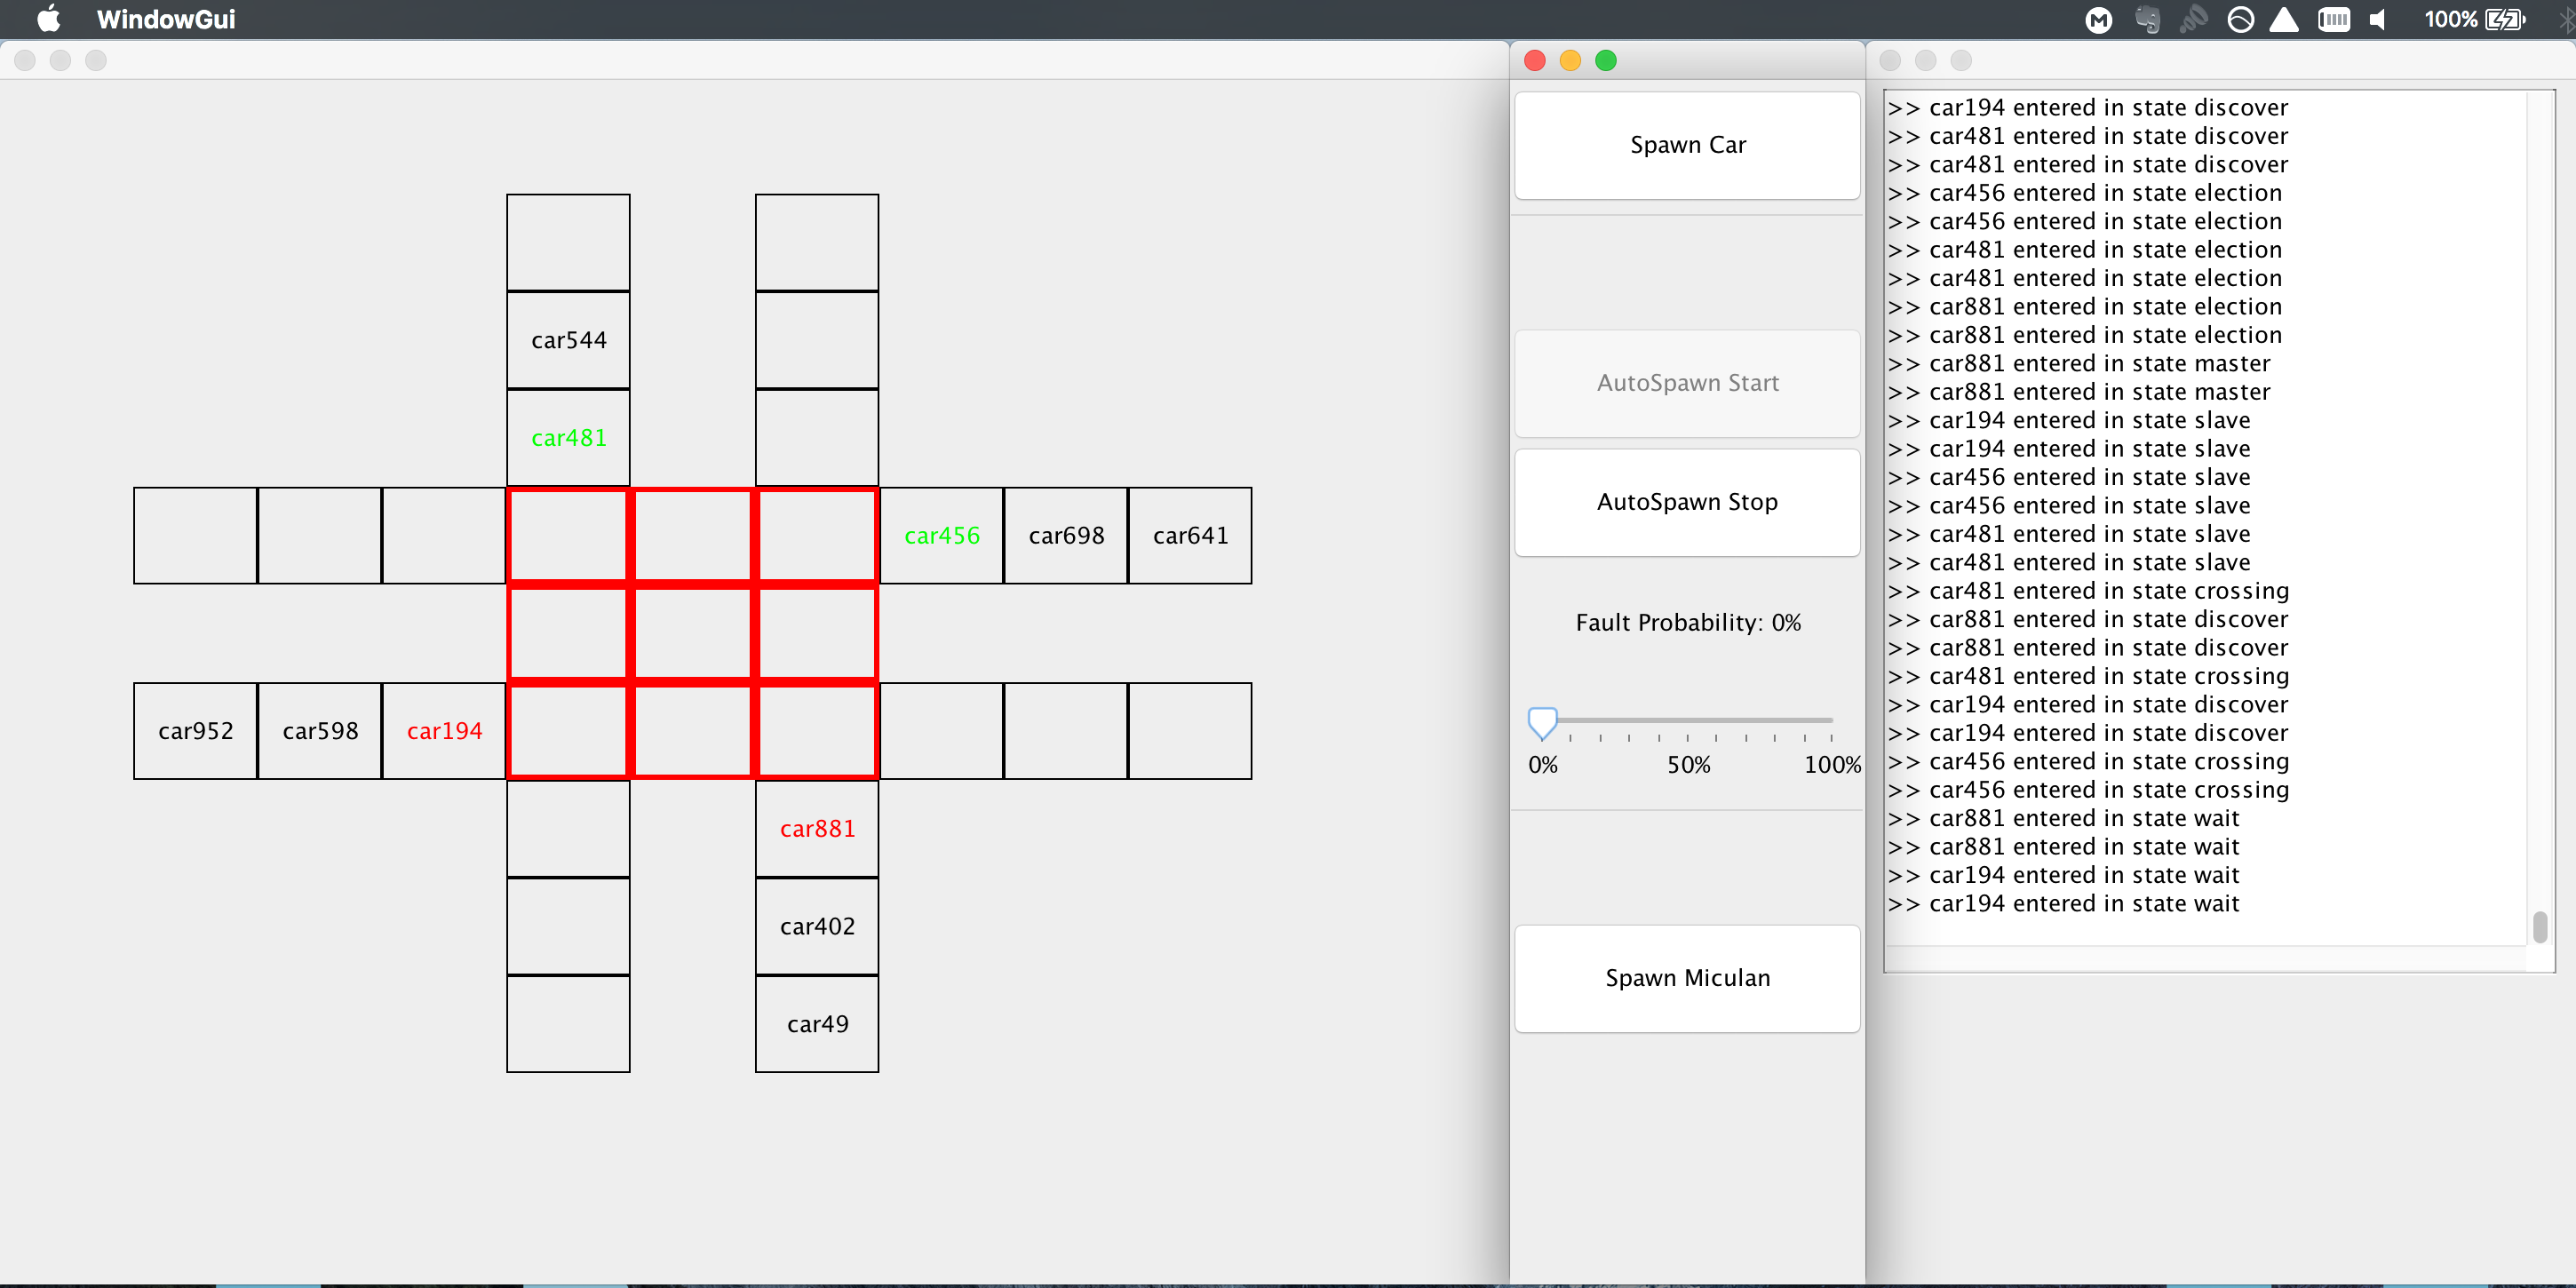
\includegraphics[width=\textwidth]{greenred}
\caption{Esempio in cui i veicoli in prossimità dell'incrocio hanno ricevuto
  messaggi \texttt{green} o \texttt{red}.}
\end{figure}

%Check if requirements from Chapter~\ref{ch:analysis} have been fulfilled.
%Quantitative tests (simulations) and screenshots of the interfaces are put here.


\chapter{Conclusioni}
La soluzione fornita implementa un sistema distribuito che risolve il problema
dell'incrocio intelligente. Nella soluzione è prevista una fase di elezione di
un leader dell'incrocio, il quale poi deciderà quali veicoli far passare.
L'algoritmo utilizzato per il coordinamento è tale da rendere la soluzione
\emph{deadlock-free} e \emph{fair}. Di default i veicoli normali partono tutti
con la stessa priorità iniziale. È possibile modellare veicoli speciali che
abbiano precedenza sugli altri (ad esempio ambulanze) semplicemente variando la
priorità iniziale.

Il sistema gestisce i casi di guasti dei veicoli: un possibile veicolo in panne
viene segnalato dai veicoli in coda chiamando il carro attrezzi. La sicurezza
stradale è garantita dalla presenza dei sensori di prossimità: un guasto di
questi ultimi è gestito come un guasto fisico; si suppone che non ci siano fault
bizantini.

Il sistema è stato implementato senza fare assunzioni sulla tipologia di
incrocio, tuttavia è stato testato solo con l'incrocio mostrato durante la
simulazione, la cui descrizione è definita all'interno del codice. Un possibile
sviluppo futuro può essere quello di scegliere un formato di descrizione
dell'incrocio e quindi permettere di caricare nella simulazione diversi tipi di
incroci.

% What has been done with respect to what has been promised in Chapters~\ref{ch:intro} and \ref{ch:analysis}, and what is left out.

\appendix

\chapter{Appendix}

Istruzioni per compilazione ed esecuzione della soluzione:
\begin{enumerate}
\item \texttt{\$ cd erlDIM} (da shell spostarsi all'interno della cartella di
  progetto)
\item \texttt{\$ chmod +x start.sh} (se non lo è già, rendere eseguibile lo
  script start.sh)
\end{enumerate}
Eseguire lo script senza parametri o con opzione -h per verificare le possibili
opzioni È necessario fornire i seguenti argomenti allo script:
\begin{itemize}
\item \texttt{-e <nome-nodo-erlang>}: indica la prima parte del nome del nodo
  erlang nel quale viene eseguito l'environment
\item \texttt{-i <indirizzo-ip>}: indica la seconda parte del nome del nodo
  erlang nel quale viene eseguito l'environment.
\end{itemize}

Se, ad esempio, si desidera eseguire l'environment su una macchina utilizzando
una scheda di rete con ip \texttt{192.168.1.100} è necessario lanciare il
seguente comando: \texttt{./start.sh -e envnode -i "192.168.1.100"}

Se la creazione del nodo erlang va a buon fine viene avviata la GUI. Come nodo
remoto e ip remoto inserire gli stessi parametri specificati sopra (nell'esempio
\texttt{envnode} e \texttt{192.168.1.100}). Come nome del nodo locale è
possibile scegliere una stringa a piacere. Come indirizzo ip locale viene invece
proposto un menù a tendina dove sono elencati tutti gli ip che la macchina ha
assegnati. Questo è l'indirizzo ip utilizzato dai veicoli e dall'environment per
inviare informazioni alla GUI. Nell'esempio, selezionare il
\texttt{192.168.1.100}.

Una volta completati tutti i campi fare click su \emph{Start} per avviare
l'interfaccia. Eventuali errori dovuti a nodi non raggiungibili o environment
non avviato vengono segnalati. Se la fase di collegamento con il nodo remoto va
a buon fine si apre l'interfaccia dalla quale gestire e monitorare
l'applicativo.

Chiudendo una qualsiasi delle finestre dell'interfaccia grafica, o inviando
\texttt{CTRL-C} dalla shell si stoppa l'applicativo.

% In the Appendix you can put code snippets, snapshots, installation instructions, etc.


%\chapter*{Evaluation}
%Your system will be judged mainly on how it operates as a distributed system. The primary evaluation will be according to whether your system has the following attributes:
%\begin{itemize}
%\item  It should be an interesting distributed system, making use of some of the algorithms we have covered in class for distributed synchronization, replication, fault tolerance and recovery, security, etc.
%\item The software should be well designed and well implemented, in terms of the overall architecture and the detailed realization.
%\item You should devise and apply systematic testing procedures, at both the unit and systems levels.
%\item The system should operate reliably and with good performance, even in the face of failures.
%\end{itemize}
%Important, but secondary considerations include:
%\begin{itemize}
%\item Time taken to do the project (the sooner the better, but do not miss details in order to end sooner)
%\item  How nice is the application's appearance: does it have a nice interface or a compelling visual display?
%\end{itemize}

\end{document}


% Local Variables:
% ispell-dictionary: "italiano"
% TeX-command-extra-options: "-shell-escape"
% End:

% LocalWords:  sensoristica timer
